\documentclass[tikz,border=10pt]{standalone}

\usepackage[T1]{fontenc}
\usepackage{lmodern}
\usepackage{xcolor}
\usetikzlibrary{arrows.meta,calc}

\definecolor{roomedge}{HTML}{6F8CA8}
\definecolor{anchorblue}{HTML}{5B7EE5}
\definecolor{anchortext}{HTML}{DEDEDE}
\definecolor{axisred}{HTML}{E84C45}
\definecolor{axisgreen}{HTML}{52A64A}
\definecolor{axisblue}{HTML}{278CE0}

\begin{document}
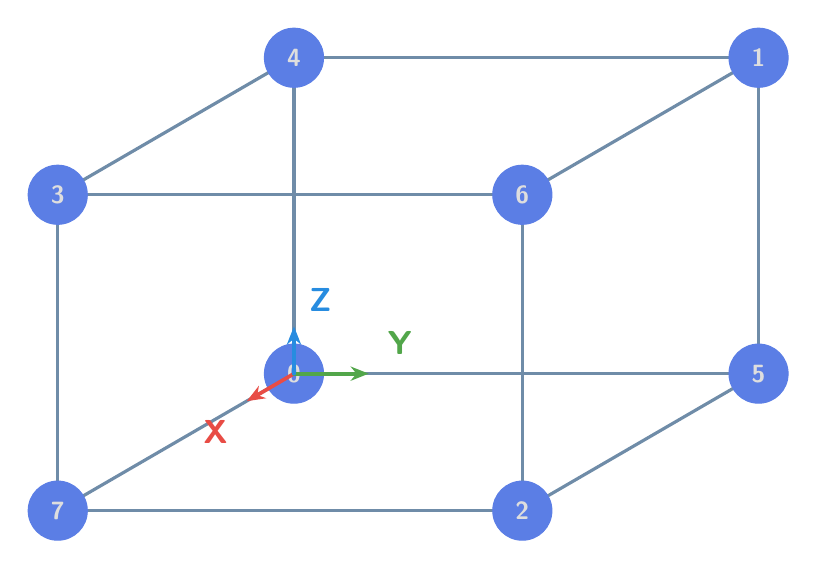
\begin{tikzpicture}[
    x={(-1.0cm,-0.58cm)},
    y={(1.18cm,0cm)},
    z={(0cm,1.18cm)},
    line cap=round,
    line join=round,
    every node/.style={font=\sffamily},
    room edge/.style={draw=roomedge,line width=1.15pt},
    anchor marker/.style={
        circle,
        fill=anchorblue,
        draw=anchorblue,
        minimum size=7.5mm,
        inner sep=0pt,
        text=anchortext,
        font=\sffamily\bfseries\small
    },
    axis X/.style={-{Stealth[length=2.3mm,width=1.8mm]},draw=axisred,line width=1.35pt},
    axis Y/.style={-{Stealth[length=2.3mm,width=1.8mm]},draw=axisgreen,line width=1.35pt},
    axis Z/.style={-{Stealth[length=2.3mm,width=1.8mm]},draw=axisblue,line width=1.35pt}
]

\coordinate (A0) at (0,0,0);
\coordinate (A7) at (3,0,0);
\coordinate (A5) at (0,5,0);
\coordinate (A2) at (3,5,0);
\coordinate (A4) at (0,0,3.4);
\coordinate (A3) at (3,0,3.4);
\coordinate (A1) at (0,5,3.4);
\coordinate (A6) at (3,5,3.4);

\draw[room edge] (A0) -- (A7);
\draw[room edge] (A0) -- (A5);
\draw[room edge] (A7) -- (A2);
\draw[room edge] (A5) -- (A2);

\draw[room edge] (A4) -- (A3);
\draw[room edge] (A4) -- (A1);
\draw[room edge] (A3) -- (A6);
\draw[room edge] (A1) -- (A6);

\draw[room edge] (A0) -- (A4);
\draw[room edge] (A7) -- (A3);
\draw[room edge] (A5) -- (A1);
\draw[room edge] (A2) -- (A6);

\node[anchor marker] at (A0) {0};
\node[anchor marker] at (A1) {1};
\node[anchor marker] at (A2) {2};
\node[anchor marker] at (A3) {3};
\node[anchor marker] at (A4) {4};
\node[anchor marker] at (A5) {5};
\node[anchor marker] at (A6) {6};
\node[anchor marker] at (A7) {7};

\draw[axis X]
    (A0) -- ([xshift=-6mm,yshift=-3.5mm]A0)
    node[below left=1mm,text=axisred,font=\sffamily\bfseries\large] {X};

\draw[axis Y]
    (A0) -- ([xshift=9.5mm,yshift=0mm]A0)
    node[above right=1mm,text=axisgreen,font=\sffamily\bfseries\large] {Y};

\draw[axis Z]
    (A0) -- ([xshift=0mm,yshift=6mm]A0)
    node[above right=0.5mm,text=axisblue,font=\sffamily\bfseries\large] {Z};

\end{tikzpicture}
\end{document}
